Dieser Abschnitt befasst sich mit den optimalen Parametern des 3DHOG, welche sich aus dem Experiment aus \cite{scherer2010histograms} ergeben hat. Außerdem wird auf ein dort eingetreten Problem bei der Gradientendefinition eingegangen.
\subsection{Parameterwahl des 3DHOG}
Das Experiment von Scherer, Walter und Schreck in \cite{scherer2010histograms} hat gezeigt, dass die Parameterwahl für den 3DHOG die Performanz stark beeinflussen kann. Eine als optimal erwiesene Einstellung ist in \figurename~\ref{Parameter} zu finden.

\begin{table}[H]
	\centering
	\caption{Optimale Parameterwahl für 3DHOG, entnommen aus \cite{scherer2010histograms}}
	\label{Parameter}
	\begin{tabular}{ll}
		Parameter                & Wert     \\
		r\textsubscript{x,y,z} & $\frac{2}{52}$    \\
		c\textsubscript{x,y,z} & 12 vxl   \\
		bins($ \theta $)       & 9        \\
		bins($ \phi $)         & 9        \\
		b\textsubscript{x,y,z} & 2 Zellen \\S
		o\textsubscript{x,y,z} & 0 Zellen \\
		Dimensionalität          & 5184    
	\end{tabular}
	
\end{table}

Der Parameter r\textsubscript{x,y,z} legt die Anzahl der Voxel im Distanzfeld fest. r\textsubscript{x,y,z} steht jeweils für die Kantenlänge jedes Voxels. Je kleiner die Kantenlänge gewählt wird, desto weniger Informationen gehen verloren, jedoch erhöht sich die Rechenzeit. Mit der Zellengröße c\textsubscript{x,y,z} stellt man ein, wie viele Gradienten in ein Histogramm aufgenommen werden. Damit lässt sich der Grad der Lokalität des Deskriptors konfigurieren \cite{scherer2010histograms}.
Mit den Parametern 	bins($ \theta $) und bins($ \phi $) bestimmt die Feinheit der Einteilungen des Histogramms. Hier hat man die Wahl zwischen Genauigkeit und Stabilität.
Die nächsten beiden Parameter legen jeweils die Größe der Blöcke (b\textsubscript{x,y,z})  und ihre Überlappung  (o\textsubscript{x,y,z}) fest. Damit wird konfiguriert, wie viele Benachbarte Zellen miteinander normalisiert werden. Diese beiden Parameter wurden entsprechend vielversprechenden Parameter aus \cite{dalal2005histograms} gewählt. Die Überlappung hatte jedoch nicht den erwarteten positiven Effekt. Deshalb wurde der Wert 0 gewählt.


\subsection{Alternative Gradientendefinition}
Durch Experimentieren hat sich herausgestellt, dass sich die zweite Ableitung für die Gradientenberechnung des 3DHOG als effektiver erwiesen hat. Scherer, Walter und Schreck \cite{scherer2010histograms} begründen es damit, dass nicht nur Informationen über Lokale Extrema in der Nähe Oberfläche des Meshes, sondern auch Informationen innerhalb des Meshs nützlich sein können. 
 \begin{figure}[thpb]
 	\centering
 	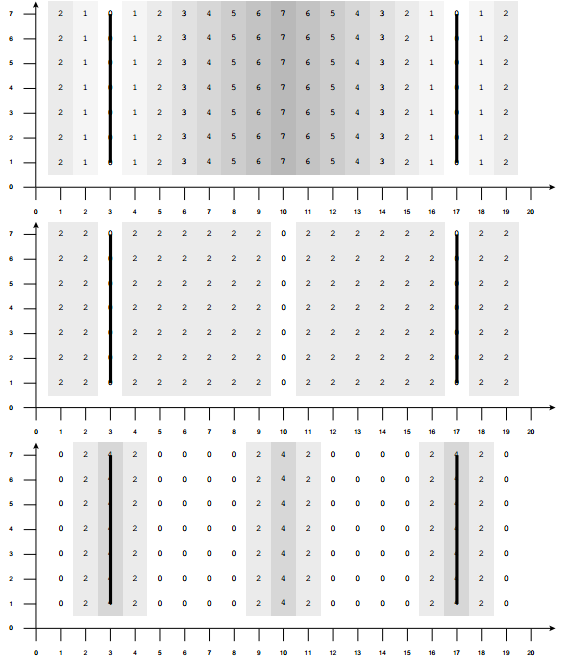
\includegraphics[width=\linewidth]{3-Diskussion/pics/2D_distance_field.png}
 	\caption{2D Darstellung eines Distanzfeldes, entnommen aus \cite{scherer2010histograms}. Das oberste Bild zeigt das eigentliche Distanzfeld, das Mittlere unter Verwendung der ersten Ableitung, das untere mit der zweiten Ableitung}
 	\label{2D_distance_field}
 \end{figure}
 Zudem liefert die ersten Ableitung nicht genau das, was man unter Gradienten in der Bildverarbeitung versteht. Einen Pixel kann man als einen Punkt in der Welt verstehen, in dem Informationen über das reflektierte Licht gespeichert werden. Der entsprechende Gradient würde z.B. an Ecken von Wänden an Stärke zunehmen. \figurename~\ref{2D_distance_field} zeigt deutlich, dass dies bei der ersten Ableitung nicht der Fall ist. Die 2. Ableitung hingegen erfüllt die Grundauffassung von Gradienten in der Bildverarbeitung.
 \newline
 
 